\section{Nested Walk-Forward Cross-Validation}
\label{app:nwfcv}

Deep learning architectures, such as \acf{LSTM} networks, Temporal Convolutional Networks (TCNs), and Spatio-Temporal Graph Neural Networks (ST-GNNs), are increasingly applied to complex panel datasets. These datasets, common in quantitative finance, econometrics, epidemiology, and meteorology, consist of multiple entities (the cross-section) observed over multiple time steps.

\medskip

When training these high-capacity models, practitioners face two primary forms of data leakage:
\begin{enumerate}
	\item \textbf{Temporal leakage (look-ahead bias):} utilizing future information to predict past or present states.
	\item \textbf{Cross-sectional leakage:} normalizing or scaling data using aggregate statistics that include testing periods across different entities.
\end{enumerate}

To rigorously evaluate generalization, the validation scheme must respect the strict arrow of time while accommodating the cross-sectional dimension. The Nested Walk-Forward Cross-Sectional Validation method is designed for this purpose, providing a conservative and realistic estimate of how a model will perform in a sequential production environment. The approach combines rolling-origin evaluation for time-series forecasting \citep{hyndman2021forecasting} with the principle that hyperparameter selection and final performance estimation must be performed on separate data \citep{cawley2010overfitting}.

\subsection{Theoretical Foundation}

\paragraph{Standard Validation versus Temporal Realities}
In standard machine learning, $k$-fold cross-validation randomly partitions the dataset into $k$ subsets, iteratively using $k-1$ folds for training and one for testing. For panel data, random shuffling destroys temporal autocorrelation and allows the model to access information from future periods. Even grouped $k$-fold validation, which keeps observations from the same entity together, does not respect the temporal ordering of the data and therefore cannot account for regime shifts or non-stationarity over time. In financial applications, these violations are especially consequential because overlapping forward-looking labels and low signal-to-noise ratios can produce misleadingly strong in-sample results \citep{lopezdeprado2018advances}.

\begin{table}[H]
	\footnotesize
	\centering
	\caption{\small Comparison of Validation Methods for Panel Data}
	\label{tab:comparison}
	\begin{tabular}{@{}lcccc@{}}
		\toprule
		\textbf{Method}              & \textbf{Time-respected?} & \textbf{Unbiased HP tuning?} & \textbf{Cross-section intact?} & \textbf{Cost} \\
		\midrule
		Standard $k$-fold            & No                       & No                           & Broken                         & Low           \\
		Grouped $k$-fold             & No                       & No                           & Intact                         & Low           \\
		Simple walk-forward          & Yes                      & No                           & Intact                         & Medium        \\
		\textbf{Nested walk-forward} & \textbf{Yes}             & \textbf{Yes}                 & \textbf{Intact}                & \textbf{High} \\
		\bottomrule
	\end{tabular}
\end{table}

\paragraph{Walk-Forward Validation}
Walk-forward validation, also known as rolling-origin evaluation or backtesting, ensures that the training set strictly precedes the validation or test set chronologically \citep{pardo2008evaluation}. Let the dataset be indexed by time $t \in \{1,2,\dots,T\}$. A walk-forward setup evaluates the model at time $t$ using only data from $1$ to $t-1$ (expanding window) or from $t-w$ to $t-1$ (rolling window of size $w$). This structure emulates the repeated retraining and prediction process that would occur in live deployment.

\paragraph{The Necessity of the Nested Approach}
Deep learning models possess numerous hyperparameters, including learning rate, dropout rate, number of layers, embedding dimensions, and window lengths. If a simple walk-forward procedure uses the validation period both to select hyperparameters and to report final performance, the resulting metrics are optimistically biased. This phenomenon, known as \textit{overfitting to the validation set}, arises because repeated model selection on the same validation data effectively incorporates information about that data into the modeling pipeline \citep{cawley2010overfitting}.

\medskip

A nested approach addresses this problem by strictly separating hyperparameter selection from out-of-sample performance estimation through two distinct, temporally ordered loops:

\begin{itemize}
	\item \textbf{Inner loop (hyperparameter optimization):} This loop operates entirely within the training window of the current outer step. It performs its own chronological walk-forward validation across multiple historical folds. For a given hyperparameter configuration, the model is trained and evaluated sequentially, and the average validation performance determines the configuration’s fitness. Because every inner validation set precedes the corresponding outer test set, the selected hyperparameters contain no look-ahead information about the subsequent out-of-sample period \citep{cawley2010overfitting, kodeli2022time}.

	\item \textbf{Outer loop (unbiased evaluation):} The outer loop simulates sequential deployment over time. Once the inner loop identifies the best hyperparameter configuration, a new model is trained using that configuration on all historical data available up to the outer test date. The model is then evaluated on strictly future observations. Advancing the outer window through time produces a sequence of genuinely out-of-sample predictions, whose aggregation provides a realistic estimate of end-to-end pipeline performance \citep{pardo2008evaluation, hyndman2021forecasting}.
\end{itemize}

\begin{figure}[H]
	\centering
	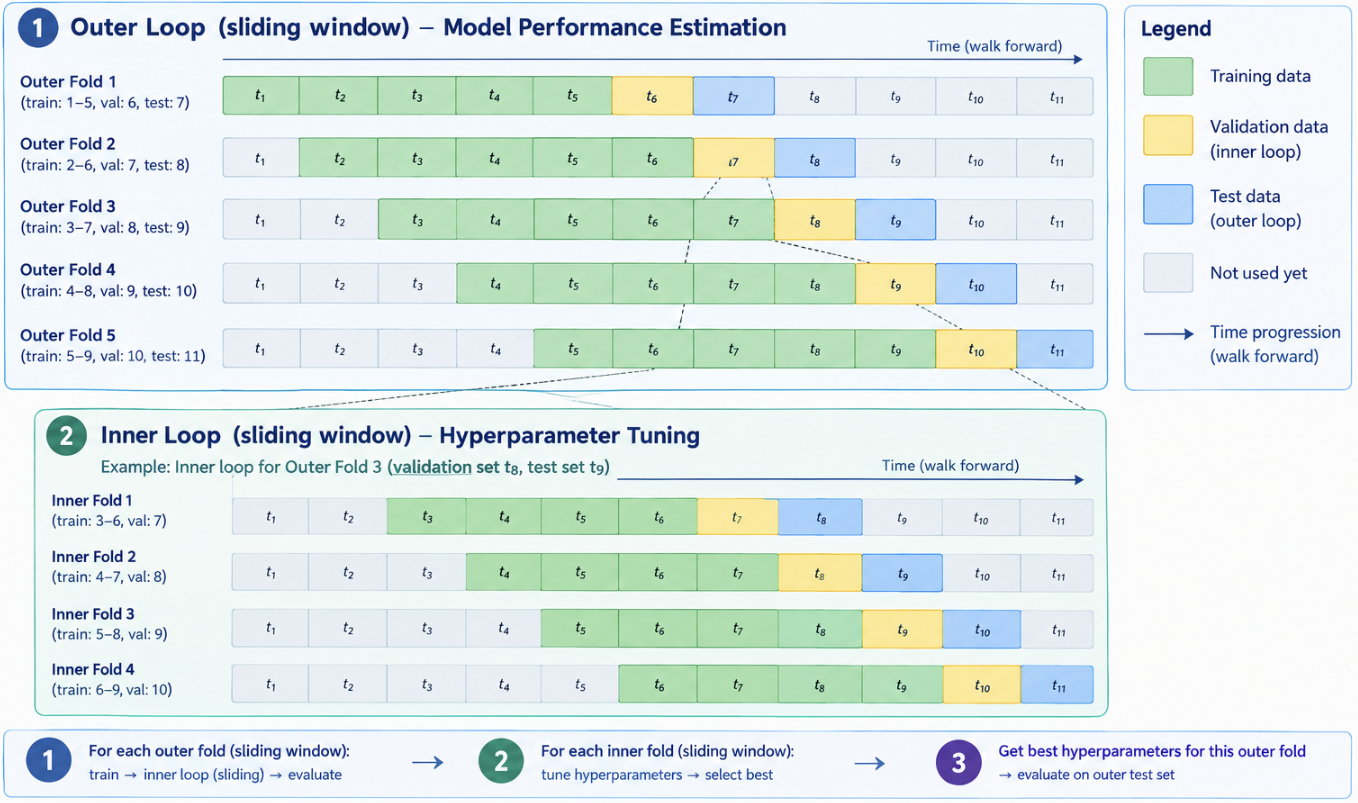
\includegraphics[width=\textwidth]{images/NWFCV.png}
	\caption{Walk-Forward Cross-Sectional Validation Visualization}
	\label{fig:NWFCV}
\end{figure}

\subsubsection*{Leakage Control for Overlapping Financial Labels}
When the target variable is a multi-period forward return or another overlapping label, temporal separation of training and test dates alone may not eliminate leakage. In that case, training observations whose label horizons overlap the validation or test interval should be removed through purging, and an embargo period may be added after the training window to attenuate serial dependence across adjacent periods \citep{lopezdeprado2018advances}. These safeguards should be applied consistently in both the inner and outer loops. A nested walk-forward implementation of this type has been used in cross-sectional equity-return prediction, where an outer walk-forward loop evaluates performance year by year while an inner leave-one-year-out procedure selects the regularization parameter using only prior-year data \citep{kodeli2022time}.

\subsection{Formal Specification}

\subsubsection{Mathematical Formulation}

\begin{algorithm}[H]
	\captionsetup{font=small}
	\caption{Nested Walk-Forward Cross-Sectional Validation Pseudocode}
	\begin{algorithmic}[1]\footnotesize
		\Require Dataset $\mathcal{D}$ sorted by time $t$, hyperparameter search space $H$, initial training window $W_{\mathrm{init}}$, step size $S$.
		\State $E_{\mathrm{OOS}} \gets []$ \Comment{Out-of-sample errors}
		\For{$T_{\mathrm{test}} = W_{\mathrm{init}}$ \textbf{to} $T$ \textbf{step} $S$}
		\State $\mathcal{D}_{\mathrm{outer\_train}} \gets \mathcal{D}[:T_{\mathrm{test}}-1]$
		\State $\mathcal{D}_{\mathrm{outer\_test}} \gets \mathcal{D}[T_{\mathrm{test}}:T_{\mathrm{test}}+S-1]$
		\State $best\_h \gets \mathrm{null}$, $min\_val\_loss \gets \infty$

		\For{$h \in H$} \Comment{Inner loop: hyperparameter tuning}
		\State $val\_loss \gets 0$
		\State Define chronological inner validation splits within $\mathcal{D}_{\mathrm{outer\_train}}$
		\For{each inner split $(\mathcal{D}_{\mathrm{inner\_train}}, \mathcal{D}_{\mathrm{inner\_val}})$}
		\State $\theta \gets \mathrm{InitializeWeights}()$
		\State $\theta \gets \mathrm{TrainDeepModel}(\mathcal{D}_{\mathrm{inner\_train}}, \theta, h)$
		\State $val\_loss \gets val\_loss + \mathrm{EvaluateCrossSection}(\mathcal{D}_{\mathrm{inner\_val}}, \theta)$
		\EndFor
		\State $val\_loss \gets val\_loss / \mathrm{number\_of\_inner\_splits}$
		\If{$val\_loss < min\_val\_loss$}
		\State $min\_val\_loss \gets val\_loss$
		\State $best\_h \gets h$
		\EndIf
		\EndFor

		\State \Comment{Outer loop: final training and evaluation}
		\State $\theta_{\mathrm{final}} \gets \mathrm{InitializeWeights}()$
		\State $\theta_{\mathrm{final}} \gets \mathrm{TrainDeepModel}(\mathcal{D}_{\mathrm{outer\_train}}, \theta_{\mathrm{final}}, best\_h)$
		\State $err \gets \mathrm{EvaluateCrossSection}(\mathcal{D}_{\mathrm{outer\_test}}, \theta_{\mathrm{final}})$
		\State $E_{\mathrm{OOS}}.\mathrm{append}(err)$
		\EndFor
		\State \Return $\mathrm{Mean}(E_{\mathrm{OOS}})$
	\end{algorithmic}
\end{algorithm}
Consider a panel dataset $\mathcal{D} = \{(\mathbf{x}_{i,t}, y_{i,t})\}$, where $i \in \{1,\dots,N\}$ denotes the cross-sectional entity and $t \in \{1,\dots,T\}$ denotes the time step. Here, $\mathbf{x}_{i,t} \in \mathbb{R}^d$ is the feature vector and $y_{i,t}$ is the target variable.

\medskip

Let $H$ be the set of candidate hyperparameter configurations, and let the outer test dates be $T_{\mathrm{test}}^{(1)}, T_{\mathrm{test}}^{(2)}, \dots, T_{\mathrm{test}}^{(K)}$.

\medskip

For the $k$-th outer fold at time $T_{\mathrm{test}}^{(k)}$:
\begin{enumerate}[topsep=0pt, itemsep=0pt, parsep=0pt]
	\item \textbf{Outer training window:} The available data are
	      \begin{equation}
		      \mathcal{D}_{\mathrm{train}}^{(k)}
		      =
		      \left\{
		      (\mathbf{x}_{i,t}, y_{i,t})
		      \mid
		      t < T_{\mathrm{test}}^{(k)}
		      \right\}.
	      \end{equation}

	\item \textbf{Inner loop (hyperparameter optimization):}
	      Split $\mathcal{D}_{\mathrm{train}}^{(k)}$ into further chronological sub-windows. Let the inner test dates be $\tau^{(1)}, \tau^{(2)}, \dots, \tau^{(J)}$, where $\tau^{(j)} < T_{\mathrm{test}}^{(k)}$. For each hyperparameter configuration $h \in H$,
	      \begin{equation}
		      \mathrm{Score}(h)
		      =
		      \dfrac{1}{J}
		      \sum_{j=1}^{J}
		      \mathcal{L}
		      \left(
		      \mathcal{M}_h
		      \left(
		      \mathcal{D}_{\mathrm{train},\tau^{(j)}}
		      \right),
		      \mathcal{D}_{\mathrm{test},\tau^{(j)}}
		      \right),
		      \label{eq:inner-score}
	      \end{equation}
	      where $\mathcal{M}_h$ is the model trained with hyperparameters $h$ and $\mathcal{L}$ is a cross-sectional loss, such as mean squared error or cross-entropy computed across all $N$ entities at time $\tau^{(j)}$. The selected configuration is
	      \begin{equation}
		      h_{\mathrm{opt}}^{(k)}
		      =
		      \arg\min_{h \in H}
		      \mathrm{Score}(h).
	      \end{equation}

	\item \textbf{Outer loop (evaluation):}
	      The final model is trained on the full outer training window using the selected configuration:
	      \begin{equation}
		      \mathcal{M}_{\mathrm{final}}^{(k)}
		      =
		      \mathrm{Train}
		      \left(
		      \mathcal{D}_{\mathrm{train}}^{(k)},
		      h_{\mathrm{opt}}^{(k)}
		      \right).
		      \label{eq:final-model}
	      \end{equation}
	      Its out-of-sample performance is evaluated on the cross-section at $T_{\mathrm{test}}^{(k)}$:
	      \begin{equation}
		      \mathrm{Error}^{(k)}
		      =
		      \mathcal{L}
		      \left(
		      \mathcal{M}_{\mathrm{final}}^{(k)},
		      \left\{
		      (\mathbf{x}_{i,T_{\mathrm{test}}^{(k)}},
		      y_{i,T_{\mathrm{test}}^{(k)}})
		      \right\}_{i=1}^{N}
		      \right).
		      \label{eq:outer-error}
	      \end{equation}
\end{enumerate}

The final estimate of generalization performance is obtained by aggregating $\mathrm{Error}^{(k)}$ across all outer folds. Because each evaluation uses a model trained and tuned exclusively on earlier data, the resulting metric reflects the expected performance of the complete modeling pipeline under sequential deployment \citep{hyndman2021forecasting, pardo2008evaluation}.

\subsubsection{Quantitative Finance Mathematical Formulation}
To adapt Nested Walk-Forward Cross-subSectional Validation to systematic trading and quantitative portfolio construction, market microstructure dynamics and risk constraints are explicitly formalized below.

\paragraph{Cross-Sectional Alpha Optimization}
Let $\mathbf{r}_{t+1} \in \mathbb{R}^N$ denote the forward return vector for an asset universe $\mathcal{U} = \{1, \dots, N\}$ at timestamp $t$. The neural network $f_\theta: \mathbb{R}^{N \times d} \to \mathbb{R}^N$ maps asset features $\mathbf{X}_t$ to predicted alpha scores $\mathbf{\hat{r}}_{t+1} = f_\theta(\mathbf{X}_t)$.

\begin{definition}[Cross-Sectional Z-Score Operator]
	For any vector $\mathbf{v} \in \mathbb{R}^N$, the cross-sectional normalization operator $\mathbf{Z}: \mathbb{R}^N \to \mathbb{R}^N$ is defined as:
	\begin{equation}
		\mathbf{Z}(\mathbf{v}) = \dfrac{v - \bar{v}}{\sigma_{\mathbf{v}}}, \quad \bar{v} = \dfrac{1}{N}\sum_{i=1}^N v_i, \quad \sigma_{\mathbf{v}} = \sqrt{\dfrac{1}{N}\sum_{i=1}^N (v_i - \bar{v})^2}
	\end{equation}
\end{definition}

\begin{definition}[Differentiable Information Coefficient Loss]
	The network optimizes the cross-sectional Pearson correlation (Information Coefficient) between predicted rankings and realized forward returns:
	\begin{equation}
		\mathcal{L}_{\text{IC}}(\theta; \mathbf{X}_t, \mathbf{r}_{t+1}) = - \dfrac{1}{N} \mathbf{Z}\left(f_\theta(\mathbf{X}_t)\right)^\top \mathbf{Z}\left(\mathbf{r}_{t+1}\right)
	\end{equation}
\end{definition}

\paragraph{Purging and Embargo Operators}
For an $h$-period forward return target $y_{i,t} = \displaystyle\prod_{k=1}^h (1 + r_{i,t+k}) - 1$, overlapping target horizons introduce non-zero temporal covariance across model residuals.
\begin{definition}[Information Leakage Sets]
	Given an inner validation set $\mathcal{T}_{\text{val}} = [t_{\text{v,start}}, t_{\text{v,end}}]$ and an embargo horizon $e \ge h$:
	\begin{align}
		\text{Purged Set: } \mathcal{P}(\mathcal{T}_{\text{val}})     & = \{ t \mid t_{\text{v,start}} - h + 1 \le t < t_{\text{v,start}} \} \\
		\text{Embargo Set: } \mathcal{E}(\mathcal{T}_{\text{val}}, e) & = \{ t \mid t_{\text{v,end}} < t \le t_{\text{v,end}} + e \}
	\end{align}
	The strictly admissible training set $\mathcal{T}_{\text{train}}^{\text{admissible}}$ is given by:
	\begin{equation}
		\mathcal{T}_{\text{train}}^{\text{admissible}} = \mathcal{T}_{\text{hist}} \setminus \left( \mathcal{T}_{\text{val}} \cup \mathcal{P}(\mathcal{T}_{\text{val}}) \cup \mathcal{E}(\mathcal{T}_{\text{val}}, e) \right)
	\end{equation}
\end{definition}

\paragraph{Inner Loop Hyperparameter Selection Objective}
To avoid validation overfit under a low signal-to-noise ratio ($\text{SNR} \ll 1$), the inner-loop hyperparameter fitness function $g(h)$ evaluates risk-adjusted portfolio performance across $J$ inner folds:
\begin{equation}
	h_{\text{opt}}^{(k)} = \arg\max_{h \in H} \dfrac{1}{J} \sum_{j=1}^J \left[ \dfrac{\mu_{\text{IC}}(h, j)}{\sigma_{\text{IC}}(h, j) + \epsilon} + \lambda \cdot \text{Sharpe}\left( \mathbf{w}_t^*(f_{\theta_{h,j}}) \right) \right]
\end{equation}
where portfolio weights $\mathbf{w}_t^* \in \mathbb{R}^N$ solve the mean-variance transaction-cost constrained problem:
\begin{equation}
	\mathbf{w}_t^*(\mathbf{\hat{r}}_{t+1}) = \arg\max_{\mathbf{w} \in \mathcal{W}} \left( \mathbf{w}^\top \mathbf{\hat{r}}_{t+1} - \dfrac{\gamma}{2} \mathbf{w}^\top \boldsymbol{\Sigma}_t \mathbf{w} - \kappa \|\mathbf{w} - \mathbf{w}_{t-1}\|_1 \right)
\end{equation}

\paragraph{Regime Drift Regularization via Proximal Updates}
To reduce computational burden while adapting to market regime changes, outer model weights $\theta^{(k)}$ undergo proximal updating from step $k-1$:
\begin{equation}
	\theta^{(k)} = \arg\min_{\theta} \left( \sum_{t \in \mathcal{D}_{\text{outer}}^{(k)}} \mathcal{L}_{\text{IC}}(\theta; \mathbf{X}_t, \mathbf{r}_{t+1}) + \dfrac{\mu}{2} \left\| \theta - \theta^{(k-1)} \right\|_{\mathbf{F}}^2 \right)
\end{equation}
where $\|\mathbf{v}\|_{\mathbf{F}}^2 = \mathbf{v}^\top \mathbf{F} \mathbf{v}$, and $\mathbf{F} = \mathbb{E}\left[ \nabla_\theta \mathcal{L} \left(\nabla_\theta \mathcal{L}\right)^\top \right]$ is the diagonal Fisher Information Matrix.

\subsection{Conclusion}
The Nested Walk-Forward Cross-Sectional Validation method is a rigorous framework for developing deep learning models on time-series panel data, where temporal leakage can invalidate performance estimates. By structurally separating hyperparameter search in the inner loop from temporal out-of-sample evaluation in the outer loop, and by evaluating errors across the cross-sectional dimension, it provides robust and realistic performance metrics \citep{cawley2010overfitting, pardo2008evaluation}. Although computationally expensive, the procedure is particularly valuable in applications such as algorithmic trading, macroeconomic forecasting, epidemiology, and personalized medicine, where deployment decisions depend on reliable estimates of future performance \citep{lopezdeprado2018advances, hyndman2021forecasting}.